\documentclass[13pt,largemargins]{homework}

\usepackage{lipsum}
\usepackage{amssymb}
\usepackage[utf8]{inputenc}
\usepackage{lmodern}
\usepackage{amsfonts}
\usepackage{hyperref}
\usepackage{bbm}
\usepackage{amsmath}
\usepackage{epstopdf}
\usepackage{enumitem}
\usepackage{subcaption}
\usepackage{bbm}
\usepackage{graphicx}
\usepackage{listings}
\usepackage{mcode}

\lstset{language=Matlab,%
basicstyle=\footnotesize\ttfamily,
numbers=left,
numberstyle=\tiny,
stepnumber=2,
frame=lines
}
\setcounter{MaxMatrixCols}{15}


\begin{document}
\section %ESERCIZIO 3
\begin{enumerate}[label=(\alph*)]
%inserire grafo ???
\item %3a
Il grafo in questione è indiretto e aciclico. Il vettore dei vertici, ordinati in ordine alfabetico, risulta essere:
\begin{gather*}
v = \{ Acciaiuoli, Albizzi, Barbadori, Bischeri, Castellani,\\
Ginori, Guadagni, Lamberteschi, Medici, Pazzi,\\ Peruzzi, Ridolfi, Salviati, Strozzi, Tornabuoni \}\\
\end{gather*}

Si procede pertanto scrivendo la matrice di adiacenza \(W\) ed il vettore dei gradi \(w_i\). 

\[W=\begin{bmatrix}
	0 & 0 & 0 & 0 & 0 & 0 & 0 & 0 & 1 & 0 & 0 & 0 & 0 & 0 & 0\\
	0 & 0 & 0 & 0 & 0 & 1 & 1 & 0 & 1 & 0 & 0 & 0 & 0 & 0 & 0\\
	0 & 0 & 0 & 0 & 1 & 0 & 0 & 0 & 1 & 0 & 0 & 0 & 0 & 0 & 0\\
	0 & 0 & 0 & 0 & 0 & 0 & 1 & 0 & 0 & 0 & 1 & 0 & 0 & 1 & 0\\
	0 & 0 & 1 & 0 & 0 & 0 & 0 & 0 & 0 & 0 & 1 & 0 & 0 & 1 & 0\\
	0 & 1 & 0 & 0 & 0 & 0 & 0 & 0 & 0 & 0 & 0 & 0 & 0 & 0 & 0\\
	0 & 1 & 0 & 1 & 0 & 0 & 0 & 1 & 0 & 0 & 0 & 0 & 0 & 0 & 1\\
	0 & 0 & 0 & 0 & 0 & 0 & 1 & 0 & 0 & 0 & 0 & 0 & 0 & 0 & 0\\
	1 & 1 & 1 & 0 & 0 & 0 & 0 & 0 & 0 & 0 & 0 & 1 & 1 & 0 & 1\\
	0 & 0 & 0 & 0 & 0 & 0 & 0 & 0 & 0 & 0 & 0 & 0 & 1 & 0 & 0\\
	0 & 0 & 0 & 1 & 1 & 0 & 0 & 0 & 0 & 0 & 0 & 0 & 0 & 1 & 0\\
	0 & 0 & 0 & 0 & 0 & 0 & 0 & 0 & 1 & 0 & 0 & 0 & 0 & 1 & 0\\
	0 & 0 & 0 & 0 & 0 & 0 & 0 & 0 & 1 & 1 & 0 & 0 & 0 & 0 & 0\\
	0 & 0 & 0 & 1 & 1 & 0 & 0 & 0 & 0 & 0 & 1 & 1 & 0 & 0 & 0\\
	0 & 0 & 0 & 0 & 0 & 0 & 1 & 0 & 1 & 0 & 0 & 0 & 0 & 0 & 0
	\end{bmatrix}\]
	
	\begin{gather*}
	\omega_i = (1, 3, 2, 3, 3, 1, 4, 1, 6, 1, 3, 2, 2, 4, 2)\\
	\end{gather*}
La misura di centralità invariante è unica e vale: 
\begin{gather*}
	\pi_i = ( \frac{1}{38}, \frac{3}{38}, \frac{1}{19}, \frac{3}{38}, \frac{3}{38}, \frac{1}{38}, \frac{2}{19}, \frac{1}{38}, \frac{3}{19}, \frac{1}{38}, \frac{3}{38}, \frac{1}{19}, \frac{1}{19}, \frac{2}{19}, \frac{1}{19} ).\\
\end{gather*}
	
	Essendo il grafo fortemente connesso e aperiodico si può concludere che la dinamica di averaging di French-De Groot converge al valore di consenso come nell'esercizio precedente: 
\[\lim_{t \to \infty}x_i(t)=\pi ' x(0)= \sum_i 	\pi_i x_i(0), \forall x(0)\] e pertanto, essendo $x(0)=[0,0,0,0,0,0,0,0,1,0,0,0,0,-1,0]'$ il vettore delle condizioni iniziali, si ottiene che il valore finale di consenso vale: 
\[\lim_{t \to \infty}x_i(t)= (1)\frac{3}{19}+(-1)\frac{2}{19}=\frac{1}{19}\]

\item %3b 
%qui ci va il codice Matlab del secondo punto 
Si riporta ora il codice Matlab sviluppato per visualizzare l'evoluzione della dinamica di opinione dei nodi del grafo, avendo assegnato ai due nodi stubborn \(\{{Strozzi}, {Medici}\}\)  rispettivamente i valori -1, +1. 


\begin{lstlisting}
Families={'Acciaiuoli', 'Albizzi', 'Barbadori', 'Bischeri',
'Castellani', 'Ginori', 'Guadagni', 'Lamberteschi','Pazzi',
'Peruzzi', 'Ridolfi', 'Salviati', 'Tornabuoni',
'Strozzi', 'Medici'}'; 

%Matrice di adiacenza W
W = zeros(15); 

W(1,15) = 1; 					%Acciaiuoli
W(2,[6 7 15]) = 1; 				%Albizzi
W(3,[5 15]) = 1; 				%Barbadori
W(4,[7 10 14]) = 1; 			%Bischeri
W(5,[3 10 14]) = 1; 			%Castellani	
W(6,2) = 1; 					%Ginori
W(7,[2 4 8 13]) = 1; 			%Guadagni
W(8,7) = 1; 					%Lamberteschi
W(9,12) = 1; 					%Pazzi
W(10,[4 5 14]) = 1; 			%Peruzzi
W(11,[15 14]) = 1; 				%Ridolfi
W(12,[15 9]) = 1; 				%Salviati
W(13,[7 15]) = 1;        		%Tornabuoni
W(14,[4 5 10 11]) = 1;  		%Strozzi
W(15,[1 2 3 11 12 13]) = 1;     %Medici
		
%vettore delle opinioni iniziali
x = zeros(15,1); 
x(14) = -1; 
x(15) = 1; 

%calcolo matrice P
w=W*ones(15,1); 
D=diag(w); 
P = D\W; 

nR=13;            				%regular nodes
nS=2;             				%stubborn nodes
u = [-1, 1]';     				%vettore degli ingressi stubborn

Q = P(1:nR, 1:nR);   			%matrice P ristretta a RxR
E = P(1:nR, (nR+1):(nR+nS)); 	%matrice P ristretta a RxS

%INIZIALIZZAZIONI
cont = 0; 
cont_max = 50; 
epsilon = 1e-4; 				%valore di tolleranza
i = 1; 

x_new = zeros(nR,1); 			%vettore delle opinioni 
x_old = zeros(nR,1); 
X_i = zeros(nR, cont_max);      %matrice dei risultati


%CALCOLO PASSI DELLA DINAMICA
while(i && cont<cont_max)
   
    cont=cont+1; 
    
    %Salvo il vettore delle opinioni nella colonna di X_i corrispondente
    X_i(sub2ind(size(X_i),1:nR, repelem(cont, nR))) = x_new; 
    
    x_new = Q*x_old + E*u;
    
    if(x_new-x_old <= epsilon)
        i = 0; 
    else
        x_old = x_new; 
    end
    
end

%PLOT DELLE TRAIETTORIE 
X=zeros(nR+nS, cont); 			%matrice X completa
X(1:nR, :) = X_i( : , 1:cont); 
X(14, :) = u(1); 
X(15, :) = u(2);

for k = 1:(nR+nS)
    figure(2)
    hold on
    plot(1:cont, X(k,:),  'LineWidth', 1)
    grid on 
    ylim([-1.1 1.1])		
end

xlabel('Tempo', 'FontSize', 10)
ylabel('Opinioni', 'FontSize', 10)
title('Traiettorie delle opinioni dei nodi', 'FontSize', 13, 'FontWeight', 'bold')
legend(Families(1:k))


\end{lstlisting}


Di seguito si riporta il grafico così prodotto, dal quale si evince che già dopo $n\approx15$ iterazioni le opinioni dei singoli nodi si stabilizzano al loro valore finale.

\begin{figure}[h]
\centering
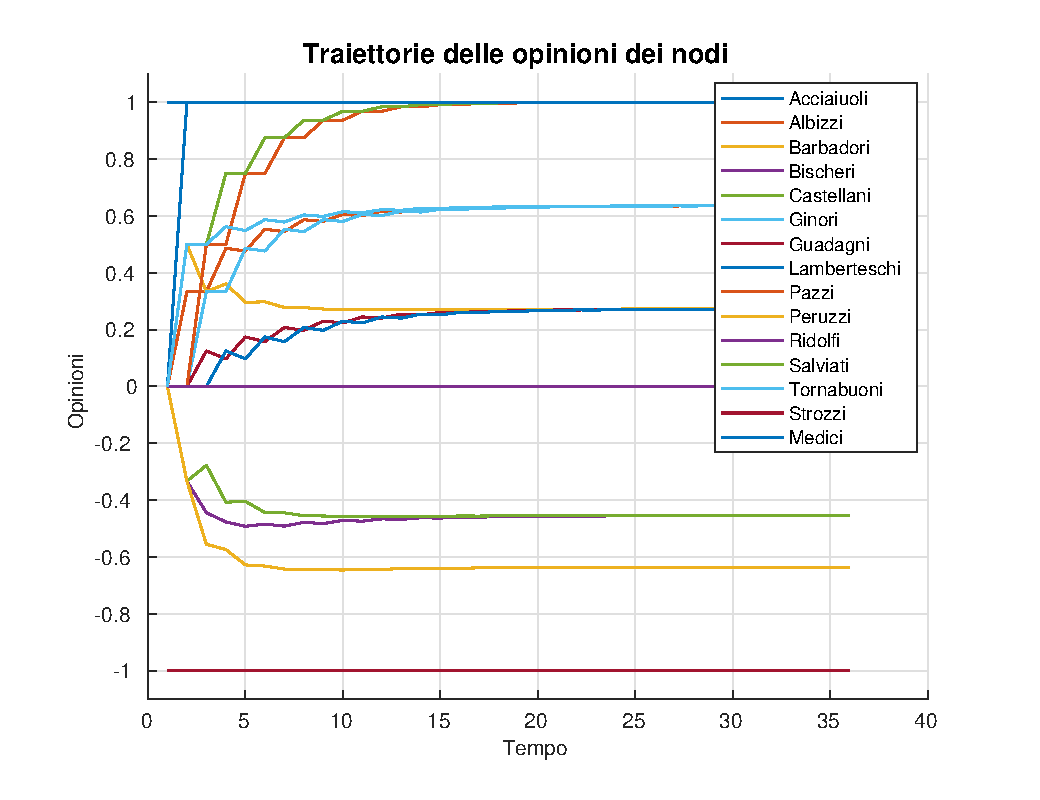
\includegraphics[scale=0.6]{traiettorie}%
\end{figure}

Il vettore di equilibrio $x(t)$ vale: 
\[x(t)=\begin{pmatrix}
    1.0000 &Acciaiuoli\\
    0.6363 &Albizzi\\
    0.2727 &Barbadori\\
   -0.4546 &Bischeri\\
   -0.4546 &Castellani\\	
    0.6362 &Ginori\\
    0.2725 &Guadagni\\
    0.2726 &Lamberteschi\\
    1.0000 &Pazzi\\
   -0.6364 &Peruzzi\\
         0 &Ridolfi\\
    1.0000 &Salviati\\
    0.6363 &Tornabuoni\\
   -1.0000 &Strozzi\\
    1.0000 &Medici   
\end{pmatrix}\]
\item%3c
L'insieme dei nodi stubborn $S=\{Castellani, Guadagni, Medici, Strozzi\}$ è globalmente raggiungibile. Sia $D=diag(\omega_i)$ e \(P\) la matrice dei pesi normalizzata
\[P=D^{-1}W=\begin{bmatrix} 
0 & 0 & 0 & 0 & 0 & 0 & 0 & 0 & 1 & 0 & 0 & 0 & 0 & 0 & 0\\
	0 & 0 & 0 & 0 & 0 & \frac{1}{3} & \frac{1}{3} & 0 & \frac{1}{3} & 0 & 0 & 0 & 0 & 0 & 0\\
	0 & 0 & 0 & 0 & \frac{1}{2} & 0 & 0 & 0 & \frac{1}{2} & 0 & 0 & 0 & 0 & 0 & 0\\
	0 & 0 & 0 & 0 & 0 & 0 & \frac{1}{3} & 0 & 0 & 0 & \frac{1}{3} & 0 & 0 & \frac{1}{3} & 0\\
	0 & 0 & \frac{1}{3} & 0 & 0 & 0 & 0 & 0 & 0 & 0 & \frac{1}{3} & 0 & 0 & \frac{1}{3} & 0\\
	0 & 1 & 0 & 0 & 0 & 0 & 0 & 0 & 0 & 0 & 0 & 0 & 0 & 0 & 0\\
	0 & \frac{1}{4} & 0 & \frac{1}{4} & 0 & 0 & 0 & \frac{1}{4} & 0 & 0 & 0 & 0 & 0 & 0 & \frac{1}{4}\\
	0 & 0 & 0 & 0 & 0 & 0 & 1 & 0 & 0 & 0 & 0 & 0 & 0 & 0 & 0\\
	\frac{1}{6} & \frac{1}{6} & \frac{1}{6} & 0 & 0 & 0 & 0 & 0 & 0 & 0 & 0 & \frac{1}{6} & \frac{1}{6} & 0 & \frac{1}{6}\\
	0 & 0 & 0 & 0 & 0 & 0 & 0 & 0 & 0 & 0 & 0 & 0 & 1 & 0 & 0\\
	0 & 0 & 0 & \frac{1}{3} & \frac{1}{3} & 0 & 0 & 0 & 0 & 0 & 0 & 0 & 0 & \frac{1}{3} & 0\\
	0 & 0 & 0 & 0 & 0 & 0 & 0 & 0 & \frac{1}{2} & 0 & 0 & 0 & 0 & \frac{1}{2} & 0\\
	0 & 0 & 0 & 0 & 0 & 0 & 0 & 0 & \frac{1}{2} & \frac{1}{2} & 0 & 0 & 0 & 0 & 0\\
	0 & 0 & 0 & \frac{1}{4} & \frac{1}{4} & 0 & 0 & 0 & 0 & 0 & \frac{1}{4} & \frac{1}{4} & 0 & 0 & 0\\
	0 & 0 & 0 & 0 & 0 & 0 & \frac{1}{2} & 0 & \frac{1}{2} & 0 & 0 & 0 & 0 & 0 & 0
\end{bmatrix}\]
Pertanto, il vettore di equilibrio della dinamica di averaging è dato dalla risoluzione del seguente sistema lineare
\begin{equation}
	\begin{cases}
		x_5 = x_7 = x_{14} = -1\\
		x_9 = +1\\
		x_i = \sum\limits_{j} P_{ij}x_j, \ j=\{1,2,3,4,6,8,10,11,12,13,15\}
	\end{cases}
\end{equation}	

\begin{equation}
	\begin{cases}
		x_5 = x_7 = x_{14} = -1\\
		x_9 = +1\\
		x_1 = x_9\\		
		x_2 = \frac{1}{3}x_6 + \frac{1}{3}x_7 + \frac{1}{3}x_9\\
		x_3 = \frac{1}{2}x_5 + \frac{1}{3}x_9\\
		x_4 = \frac{1}{3}x_7 + \frac{1}{3}x_{11} + \frac{1}{3}x_{14}\\
		x_6 = x_2\\
		x_8 = x_7\\
		x_{10} = x_{13}\\
		x_{11} = \frac{1}{3}x_4 + \frac{1}{3}x_5 + \frac{1}{3}x_{14}\\		
		x_{12} = \frac{1}{2}x_9 + \frac{1}{3}x_{14}\\
		x_{13} = \frac{1}{2}x_9 + \frac{1}{2}x_{10}\\
		x_{15} = \frac{1}{2}x_7 + \frac{1}{2}x_9\\	
	\end{cases}
\end{equation}	

La soluzione del sistema è
\begin{equation}
x(0)=[1,0,0,-1,-1,0,-1,-1,1,1,-1,0,1,-1,0]'
\end{equation}
da cui si deduce che Acciaiuoli, Pazzi e Salviati avranno la stessa opinionde dei Medici pari a $+1$ mentre Bischeri, Castellani, Guadagni, Lamberteschi, Peruzzi e Strozzi condivideranno l'opinione $-1$ ed i restanti Albizzi, Barbadori, Ginori, Ridolfi e Tornabuoni manterranno l'opinione iniziale pari a $0$.  

\item %3d 
%Page Rank centrality


\end{enumerate}

\end{document}